\chapter{Gesamtkonzept Softwareplattform}

In diesem Kapitel wird anhand der Anforderungen aus dem Forschungsansatz eine Gesamtarchitektur des Softwareplattforms vorgestellt, sowie die Softwarearchitektur der beiden Softwarekomponenten \enquote{Runtime Node} und \enquote{Runtime Master}. 

\section{Verteiltes Rechenplattform aus autonomen Fahrzeugsteuergeräten}

Die Rechenleistung von autonomen Fahrzeugen kann in verschiedenen Nutzungskonzepten verwendet werden. Im Kapitel \autoref{Hardwareumgebung in Fahrzeugen} wurde die Hardware vorgestellt, die typischerweise in autonomen Fahrzeugsteuergeräten zu finden ist. Es wird deutlich, dass diese Steuergeräte über Hardwaremodule verfügen, die die Rechenleistung für spezifische Rechenoperationen erhöhen. Grafikprozessoren beinhalten viele Rechenkerne, die parallel auf gro0en Datenmengen opreationen ausführen können. In den meisten Architekturen können die GPU-Cores nur in Gruppen verwendet werden, wobei jede Gruppe die gleiche Rechenoperation ausführen muss. Kerne für Neuronale Netzwerk Berechnungen implementieren Matrix Operationen in Hardware, so dass diese in erheblich weniger Rechenzyklen als bei sequentieller Berechnung durchgeführt werden können. Folglich können nur solche Rechenaufgaben sinnvoll auf diese Steuergeräte ausgelagert werden, die sich in viele parallele Berechnungen aufteilen lassen. Typische Beispiele für solche Berechnungen sind:

\begin{itemize}
    \item Mathematik: Vektor und Matrixoperationen
    \item Bildbearbeitung: FFT oder Faltungsoperationen
    \item Simulation: Moleküldynamik, Finite-Elemente Analyze, Fluiddynamik
    \item Finanzsegment: Monte Carlo Simulation, Optionspreisgestaltung, Portfolio Optimierung
    \item Kryptographie und Sicherheit: Hashing Algorithmen, Passwortknacken, Blockchain und Kryptowährung Mining
    \item Datenanalyse in Naturwissenschaften: Genomische und bioinformatische Berechnungen, Big Data Verarbeitung
    \item Optimerung: Genetische Algorithmen Berechnungen
    \item Quantum Computing: Simulation von Quantumsystemen
\end{itemize}

Die Neuronale Netzwerk Beschleuniger können zudem für das Trainieren von neuronalen Netzwerken effizient verwendet werden. 

Trotz der Einschränkung in der Art der Rechenaufgaben, die auf der Hardware effizient berechnet werden können, ergibt sich eine Vielzahl möglicher Anwendungsszenarien. Die ungenutzte Rechenleistung kann also von verschiedenen Kunden sinnvoll verwendet werden. Folgende Ansätze für die Bereitstellung der Ressourcen an Kunden wären Denkbar:

\begin{itemize}
    \item Nutzung ausschließlich durch den Hersteller: Diese Methode ist die transparenteste und sicherste Methode für den Fahrzeughersteller. Nur der Hersteller selber Applikationen auf die Fahrzeuge ausrollen und die ungenutzte Rechenleistung nutzen
    \item Nutzung durch Hersteller und ausgewählte Kunden: Der Hersteller stellt die Rechenleistung auch an ausgewählte Kunden zur Verfügung, hierbei vertraut der Hersteller den Kunden, dass sie keine illegale Aktivitäten ausüben und nicht aktiv Versuchen Schutzmechanismen des Systems umzugehen.
    \item Nutzung durch frei verfügbaren Marktplatz: Beliebige Kunden können auf dem Marktplatz Rechenleistung einkaufen. In diesem Konzept muss sichergestellt werden dass Kunden keine illegale Aktivitäten ausüben und dass sie die Sicherheitsmechanismen des Plattforms nicht versuchen zu umgehen.
\end{itemize}

Für die ersten Versionen eines solchen Plattforms würden realistisch nur die ersten Beiden Möglichkeiten in Frage kommen. Eine freie Nutzung erfordert sehr hohe Sicherheitsstandards für die Plattform, die mit erheblichem Entwicklungs- und Erfahrungsaufwand verbunden sind. 

Die Nutzung freier Rechenressourcen erhöht den Stromverbrauch des Fahrzeugs. Daher müssen Anreize für die Nutzer geschaffen werden, die Rechenleistung des Fahrzeugs freizugeben. Hier können ähnliche Konzepte wie in der Informatik verwendet werden. Es gibt verschiedene Plattformen, auf denen PC-Nutzer ihre Rechenleistung zur Verfügung stellen können. 

Plattformen, die auf freiwilliger Teilnahme und Bereitstellung von Rechenressourcen beruhen, haben sich als erfolgreich erwiesen. Voraussetzung ist, dass die Rechenleistung nur für Zwecke eingesetzt wird, die von der Gesellschaft als gemeinnützig und sinnvoll erachtet werden. Ein verbreitetes Beispiel ist das Projekt \gls{BOINC}. In diesem Projekt können Nutzer ihre ungenutzte Rechenleistung für verschiedene naturwissenschaftliche Projekte zur Verfügung stellen.  \gls{BOINC} stellt die Rechenleistung für verschiedene Anwendungen in Bereichen wie Medizintechnik, Biologie, Mathematik, Linguistik, Klimaforschung, Umweltwissenschaften, Astrophysik zur Verfügung. Die teilnehmenden Nutzer erhalten Punkte für die im Projekt erbrachte Rechenleistung. Diese Punkte können jedoch nicht eingelöst werden und dienen lediglich der Nachvollziehbarkeit und Vergleichbarkeit der erbrachten Rechenleistung unter den Nutzern. Ein ähnliches Konzept könnte daher auch für die Nutzung der freien Rechenleistung von Fahrzeugen erfolgreich sein, sofern die Rechenleistung für gemeinnützige Zwecke genutzt wird.

Wenn eine kommerzielle Nutzung der Rechenleistung vorgesehen ist, müssen die Nutzer, die Rechenleistung zur Verfügung stellen, entlohnt werden. Viele Plattformen im IT-Bereich setzen dabei auf die Bezahlung mit Kryptowährungen. Dies hat den Vorteil, dass die Zahlungsbedingungen direkt im Blockchain-Vertrag festgehalten werden können, sodass kein Vertrauen in die Einhaltung der Bedingungen durch den Plattformbetreiber erforderlich ist. Exemplarisch kann in diesem Kontext das Golem-Projekt betrachtet werden. 

Das Konzept sieht die Implementierung eines Markplatzes vor, wo Benutzer Rechenleistung einkaufen und verkaufen können. Die Erstellung der Rechenaufgaben kann auf zwei verschiedene Arten erfolgen. Entweder werden bereits kompatible Funktionscodes in Form von Vorlagen genutzt, oder die Funktionscodes werden vom Benutzer implementiert. Die Aufgabenverwaltung registriert die neue Aufgabe, welche durch einen Benutzer angestoßen wurde. Der Benutzer, der die Rechenleistung der Plattform in Anspruch nehmen möchte, erstellt ein Angebot, in dem er die Höhe der Vergütung angibt. Diese Angebote werden auf dem Netzwerk an allen Benutzer übertragen, die Rechenleistung zur Verfügung stellen. Zusätzlich kann das Angebot Einschränkungen bezüglich der Hardware oder geographische Lage beinhalten.

Die Bereitstellung von Rechenleistung erfolgt durch die lokalen Ausführungen eines Transaktionssystem-Moduls durch die jeweiligen Benutzer. Dieser Modul sammelt alle verfügbaren Aufgabenangebote im Netzwerk und wählt das beste Angebot aus. Des Weiteren verfügt auch derjenige, der ein Angebot erstellt, über eine Reputation auf der Plattform. Angebote von Benutzern, deren Reputation als zu gering erachtet wird, werden abgelehnt. Sofern alle Anforderungen des Angebots durch den Rechenleistung-Bereitsteller erfüllt sind, wird das Angebot angenommen. 

Die Rechenaufgabe, inklusive benötigte Ressourcen wird auf den PC vom Rechenleistung-Bereitsteller heruntergeladen. Der PC berechnet im Anschluss die entsprechende Aufgabe. Der Rechenleistung-Bereitsteller kann die geladenen Anwendungen in verschiedenen Umgebungen ausführen. Es kann eine Virtualisierungsmethode wie Container oder virtuelle Maschine verwendet werden, um die Anwendungen vom Hostsystem zu isolieren, oder es kann direkt auf dem Hostsystem ausgeführt werden, wenn die Anwendung als vertrauenswürdig eingestuft wird. 

Nach der Berechnung der Aufgabe werden die Ergebnisse und Protokolle an den Auftraggeber zurückgeschickt. Die Aufgabenverwaltung validiert die Ergebnisse, indem entweder Teile der Aufgabe von anderen Teilnehmern redundant berechnet werden oder Teile lokal berechnet und überprüft werden. Sind die Ergebnisse erfolgreich validiert, wird der Benutzer, der die Rechenleistung erbracht hat, entsprechend dem Angebot bezahlt. Falls die Ergebnisse nicht korrekt sind, wird die Reputation des Rechenleistung-Bereitstellers verringert. 

Ein Konzept wie es im Golem-Projekt umgesetzt wurde, eignet sich auch für die Bereitstellung von Fahrzeugrechenressourcen im kommerziellen Einsatz. Dieses Konzept kann vereinfacht werden, wenn die Plattform vom Hersteller betrieben wird. Der Hersteller kann eine zentrale Zahlungsinstanz betreiben, so dass keine Kryptowährung als Zahlungsmittel verwendet werden muss. In diesem Fall wird der Hersteller als vertrauenswürdiger Betreiber angesehen, der die Auszahlung pflichtgemäß ausführt. Die Überprüfung der berechneten Daten und damit die Beurteilung der Vertrauenswürdigkeit der einzelnen Teilnehmer kann stark vereinfacht oder ganz weggelassen werden. Die Software für die Steuergeräte kommt vom Hersteller, so dass ein Eingriff durch den Kunden deutlich schwieriger und unwahrscheinlicher ist. Eine Isolierung vom restlichen System ist aber auch dann sinnvoll, wenn nur der Hersteller externe Applikationen auf die Steuergeräte auslagern kann. Auch wenn ein Missbrauch ausgeschlossen werden kann, kann ein unbeabsichtigter Fehler bei unzureichender Isolierung dennoch zu einem Sicherheitsrisiko führen. 

\section{Architektur der Softwareplattform}

Die prototypische Implementierung der Plattform orientiert sich in ihrer Architektur an bestehenden Systemen aus der Informationstechnik. Wie im \autoref{Forschungsansatz} erarbeitet, besteht die Plattform aus zwei Hauptkomponenten. Die \enquote{Runtime Node} Komponente läuft auf den Fahrzeugsteuergeräten und ist im gesamten Netzwerk mehrfach vorhanden. Die Komponente \enquote{Runtime Master} ist einmal im Netzwerk vorhanden und verwaltet die \enquote{Runtime Node} Komponenten. Eine Gesamtarchitektur ist in der \autoref{architektur} dargestellt.

\begin{figure}[htbp]
	\centering
	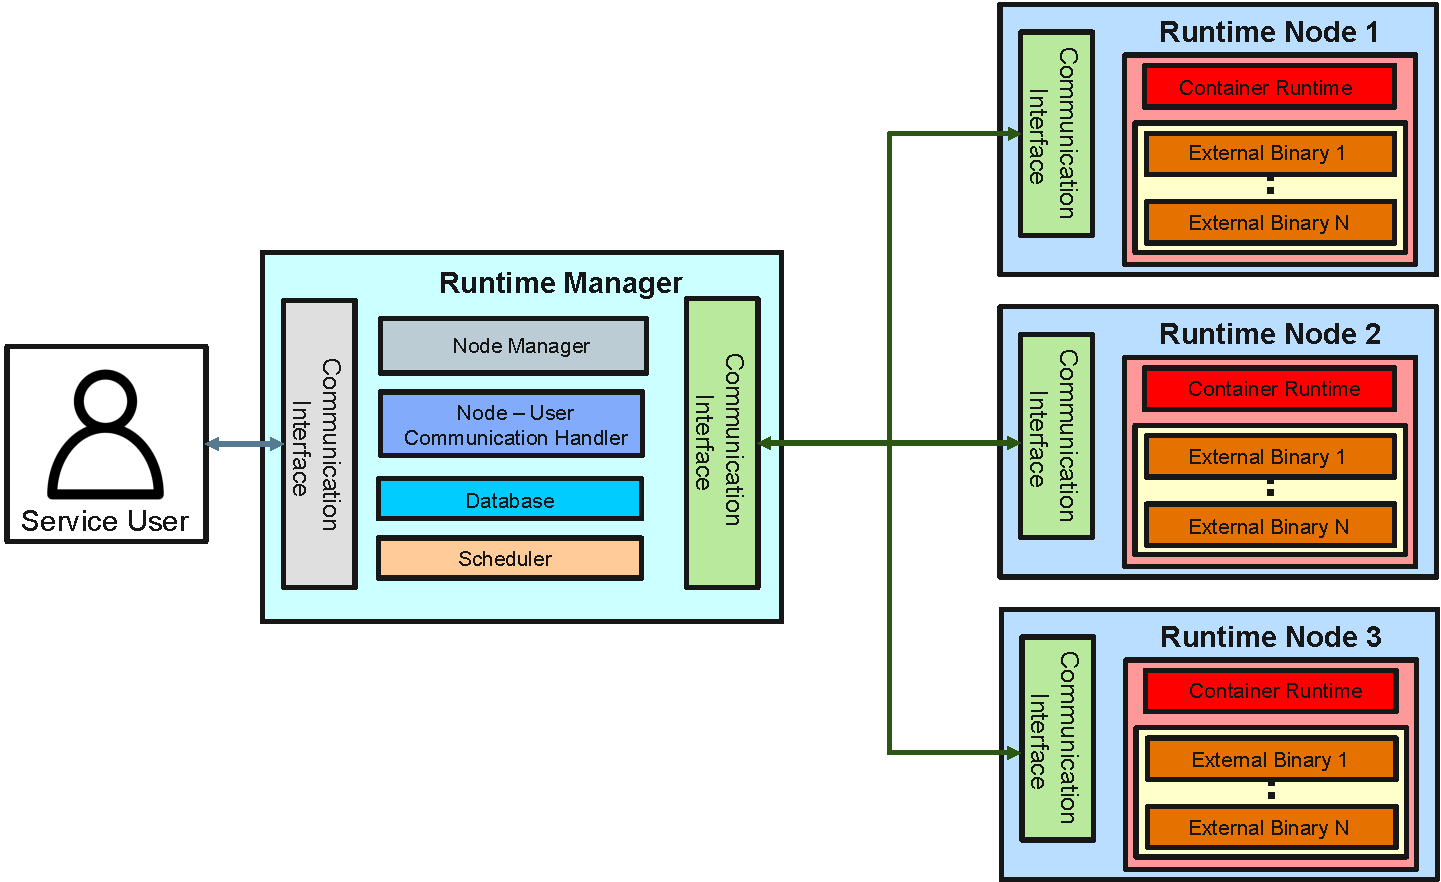
\includegraphics[width=\textwidth]{./content/graphics/Architecture.pdf}
	\caption{Gesamtarchitektur der Softwareplattform}
	\label{architektur}
\end{figure}

\subsection{Runtime Node}

Diese Komponente wird auf den Fahrzeugsteuergeräten ausgeführt und setzt sich aus mehreren Softwarekomponenten zusammen. Die Kommunikationsschnittstelle wird als eigenständige Softwarekomponente implementiert, die nicht Teil der Softwarekomponente Runtime Node ist. Diese Struktur ermöglicht einen einfachen Austausch der Kommunikationsschnittstelle und damit einen einfachen Wechsel des Kommunikationsprotokolls. Die Kommunikation zwischen der Kommunikationsschnittstelle und dem Runtime Node erfolgt über eine Interprozesskommunikationssockel. Die Informationen werden im \gls{JSON} Format übertragen. Der Runtime Node interpretiert die eingehenden Befehle mit einem JSON-Parser-Modul. Statusrückmeldungen vom Runtime Node werden ebenfalls als JSON an die Kommunikationsschnittstelle gesendet. 

\begin{figure}[htbp]
	\centering
	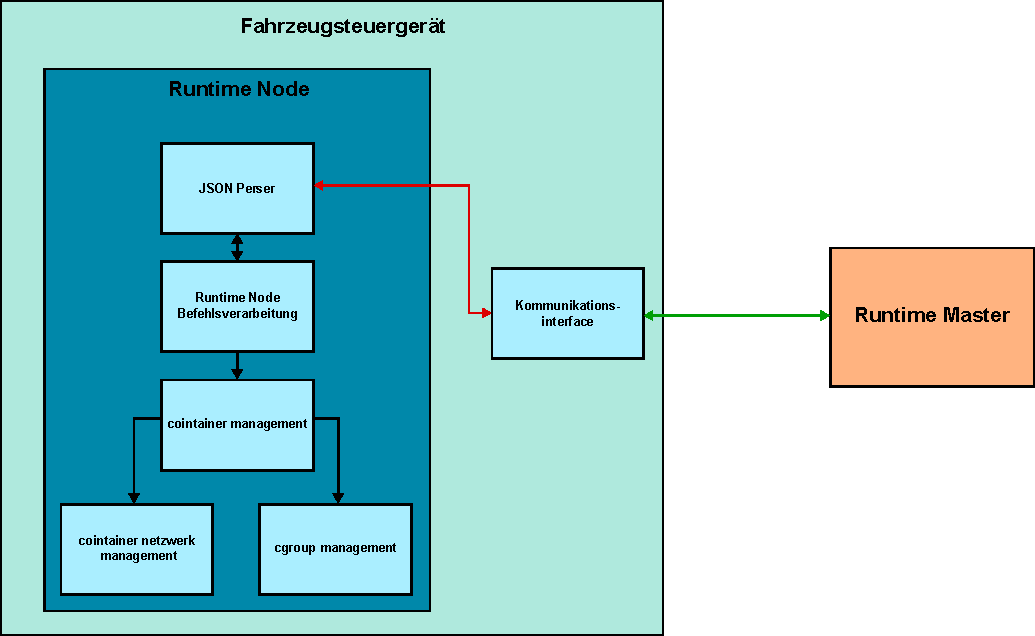
\includegraphics[width=\textwidth]{./content/graphics/Runtime_Node_Arch.pdf}
	\caption{Runtime Node Struktur}
	\label{runtime node}
\end{figure}

\subsection{Runtime Master}

\begin{figure}[htbp]
	\centering
	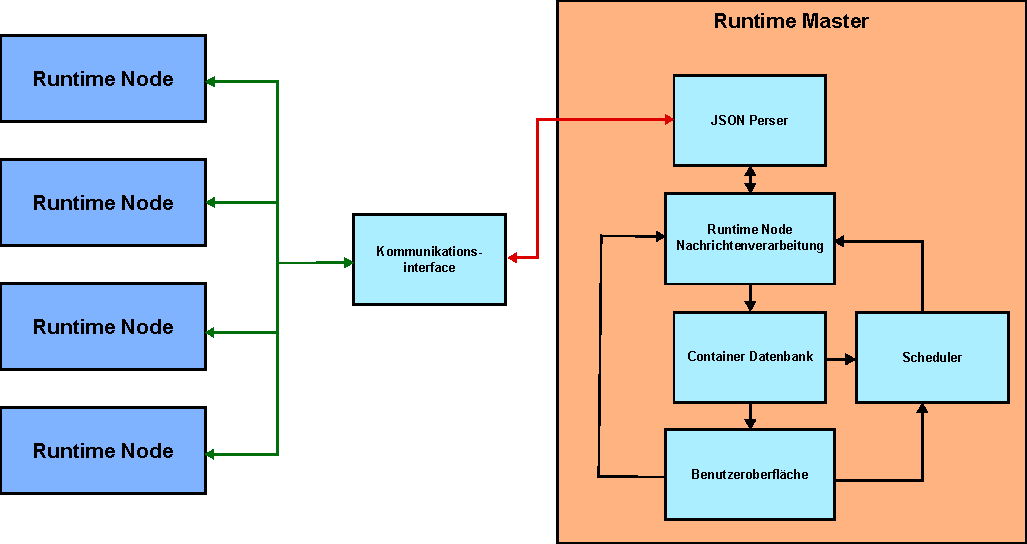
\includegraphics[width=\textwidth]{./content/graphics/Runtime_Master_Arch.pdf}
	\caption{Runtime Master Struktur}
	\label{runtime master}
\end{figure}

\subsection{Kommunikation}

Innerhalb des Systems findet Kommunikation sowohl zwischen den Fahrzeugen als auch zwischen den einzelnen Softwarekomponenten statt. Diese unterschiedlichen Kommunikationsarten stellen unterschiedliche Anforderungen an die verwendete Kommunikationsschnittstelle. Diese werden im folgenden Abschnitt dargestellt.

\subsubsection{Kommunikation zwischen Fahrzeugen und Runtime Master}

Die Fahrzeuge bilden ein verteiltes System, das von einer Runtime Master Instanz verwaltet wird. Dies entspricht einer klassischen Client/Server Kommunikationsstruktur. Die Kommunikation zwischen Fahrzeugen und Runtime Node wird voraussichtlich über eine Internetverbindung realisiert. Denkbar wäre auch ein vom Fahrzeughersteller bereitgestelltes Netzwerk, das ähnlich der Internetverbindung über das Mobilfunknetz zur Verfügung gestellt wird. In dieser Arbeit wird generell davon ausgegangen, dass sich Fahrzeuge und Runtime Master im selben Netzwerk befinden. 

Für die Client/Server Kommunikation existieren bereits verschiedene Konzepte. Die folgenden Methoden werden häufig verwendet:

\begin{itemize}
    \item Request/Response: Client sendet Anfragen an einen Server und wartet auf Antwort
    \item Publish/Subscribe: Publisher versenden Nachrichten zu einem definierten Thema. Subscriber erhalten die Nachrichten zu den Themen, die sie abonniert haben.
    \item Websocket: Duplex Kommunikation über eine \gls{TCP} Verbindung. 
    \item \gls{RPC}: Ermöglicht die Ausführung eines Prozesses auf einem anderen System, als ob es sich um ein lokales System handeln würde.
\end{itemize}

Hauptsächlich finden zwei verschiedene Kommunikationsarten zwischen Runtime Node und Runtime Master statt. Einerseits werden die Anweisungen an die Runtime Nodes über eine \gls{API} Schnittstelle vom Runtime Master übertragen, andererseits müssen die externe Applikationen an die Runtime Nodes übertragen werden. 

Die Kommunikation mit \gls{API} Schnittstellen wird häufig in Form von Request/Response über das HTTP Protokoll realisiert. Hierfür stehen zahlreiche Tools und Softwarebibliotheken zur Verfügung. Die Kommunikation kann auch verschlüsselt erfolgen. 

Das \gls{SOA} Architekturmuster gewinnt in der Informationstechnologie zunehmend an Popularität, da es die effiziente Koordination verteilter Ressourcen und die Wiederverwendbarkeit einzelner Komponenten verbessert. Dieses Muster ist auch Gegenstand der Forschung für Fahrzeugarchitekturen, da diese ebenfalls als verteilte Systeme betrachtet werden können, in denen einzelne Teilnehmer für unterschiedliche Funktionalitäten wiederverwendbar gestaltet werden müssen. Es ist davon auszugehen, dass zukünftige Fahrzeugarchitekturen diesem oder einem ähnlichen Ansatz folgen werden. Als Kommunikationsprotokoll eignet sich für \gls{SOA} Architekturen ein Protokoll, das eine lose Kopplung der einzelnen Komponenten erlaubt und die Anzahl der Teilnehmer dynamisch variieren kann. In diesen Konzepten wird häufig das Publish/Subscribe Konzept verwendet. Publisher können jederzeit Informationen zu einem bestimmten Thema veröffentlichen. Alle Subscriber, die das Thema abonniert haben, erhalten die Daten. Die Anzahl der Subscriber und Publisher kann sich während des Betriebs dynamisch ändern, Publisher können ihre Daten auch dann publizieren, wenn es von keinem Subscriber abonniert wurde. Im Gegensatz zum Request/Response Verfahren müssen sich Subscriber und Publisher nicht kennen. Dieses Konzept erlaubt somit eine lose Kopplung und einfache Skalierbarkeit der Kommunikationsteilnehmer. Viele Implementierungen von Publish/Subscribe Kommunikationsprotokollen beinhalten \gls{QoS} Regeln in den übertragenen Nachrichten. In verteilten Systemen, wie sie in \gls{SOA} Architekturen vorkommen, haben die Teilnehmer unterschiedliche Anforderungen an die übertragenen Informationen. Um potentielle Probleme bei der Mehrfachnutzung der gleichen Daten zu vermeiden, können mit Hilfe von \gls{QoS} Regeln bestimmte Garantien definiert werden. Teilnehmer, die auf die Daten zugreifen, können anhand dieser Informationen überprüfen, ob die Daten ein für ihre Funktionalitäten geeignetes Verhalten aufweisen. Je nach Implementierung kann die Anzahl der definierbaren \gls{QoS} Regeln variieren. Als Beispiel kann eine der am weitesten verbreiteten Publish/Subscribe Implementierungen namens \gls{MQTT} betrachtet werden. Diese Implementierung stellt eine \gls{QoS} Regel zur Verfügung, die definiert, wie Nachrichten an Teilnehmer übermittelt werden. Die folgenden 3 Stufen können verwendet werden:

\begin{itemize}
    \item \gls{QoS} 0: Nachricht wird höchstens einmal gesendet, Abonnenten, die zum Zeitpunkt des Sendens das Thema der Nachricht nicht abonniert haben, erhalten die Nachricht nicht.
    \item \gls{QoS} 1: Nachricht wird mindestens einmal gesendet, Nachricht wird kontinuierlich wiederholt, bis ein Teilnehmer eine Empfangsbestätigung zurücksendet.
    \item \gls{QoS} 2: Nachricht wird genau einmal übertragen. Nachricht wird zunächst im Broker zwischengespeichert und an alle Teilnehmer gesendet. Erst wenn alle Abonnenten den Empfang bestätigt haben, wird die Nachricht gelöscht und die erfolgreiche Übertragung an den Publisher gesendet. 
\end{itemize}

Bei der Konfiguration von Nachrichten kann der \gls{QoS}-Level festgelegt und damit das Übertragungsverhalten der Nachricht konfiguriert werden. Andere Implementierungen können auch mehrere definierbare \gls{QoS}-Regeln enthalten, um eine noch genauere Abstimmung der Anforderungen zwischen den Kommunikationsteilnehmern zu ermöglichen. Die Publish/Subscribe Implementierung \gls{DDS} bietet 22 konfigurierbare \gls{QoS} Regeln. Die zusätzlichen Regeln erlauben die Festlegung von weiteren Anforderungen wie maximaler Latenz, Lebensdauer oder Zuverlässigkeit der Nachrichten festzulegen. 

Publish/Subscribe-Systeme können entweder von einer zentralen Instanz, einem so genannten Broker oder Message Bus, oder ohne zentrale Instanz verwaltet werden. Wird eine zentrale Verwaltungsinstanz verwendet, verbinden sich alle Teilnehmer mit dieser Instanz. Publisher übermitteln ihre Nachrichten an diese Administration, Subscriber abonnieren Themen bei der Administration. Die Nachrichten werden entsprechend an die Abonnenten weitergeleitet. Die gesamte Kommunikation in dieser Topologie läuft über diese zentrale Instanz, diese verwaltet die Kommunikationsteilnehmer und Nachrichtenfluss.

Bei der dezentralen Umsetzung entfällt die zentrale Verwaltungsinstanz. Die Teilnehmer kommunizieren direkt miteinander, welches zwei Vorteile mit sich bringt. Zum einen erhöht sich die Robustheit des Systems durch den Wegfall der zentralen Administration, zum anderen verringert sich die Latenz und der Bandbreitenbedarf im Netzwerk durch die direkte Kommunikation. Die Komplexität wird jedoch dadurch erhöht, dass die Netzwerkteilnehmer die anderen Teilnehmer selbst entdecken 
müssen und die Publisher selbst dafür verantwortlich sind, ihre Nachrichten an alle Abonnenten zu übermitteln. Die Erkennung der Teilnehmer erfolgt durch periodische Broadcast Nachrichten, die an alle Netzwerkteilnehmer übermittelt werden. Durch diese Discovery Nachrichten werden Publisher darüber informiert, welche Netzwerkteilnehmer ihre Nachrichten Abonnieren. Die Übertragung der Nachrichten an die Abonnenten erfolgt gezielt an die Netzwerkteilnehmer die das entsprechende Thema abonnieren. Ein Nachteil dieser Methode ergibt sich aus den per Broadcast übertragenen Discovery Nachrichten. Broadcast Nachrichten werden im gesamten Netzwerk an alle Netzwerkteilnehmer verteilt. Dies kann in großen Netzwerken zu einem hohen Bandbreitenverbrauch führen. Aus diesem Grund werden Broadcasts im Internet nicht verwendet, da sie aufgrund der großen Anzahl von Geräten sehr ineffizient wären. Die dezentrale Implementierung mit Broadcast Nachrichten zur Erkennung weiterer Teilnehmer ist aus diesem Grund für die Kommunikation über das Internet nicht nutzbar. Um dieses Problem zu umgehen, bieten dezentrale Publish/Subscribe Implementierungen oft auch die Möglichkeit, Discovery Nachrichten an vorkonfigurierte Adressen zu senden. In diesem Fall müssen die Adressen allen potentiellen Teilnehmern zur Konfigurationszeit bekannt sein, so dass das Netzwerk nicht so flexibel erweiterbar ist.

In der prototypischen Implementierung wird davon ausgegangen, dass sich die serviceorientierte Architektur im Automobil durchsetzen wird, insbesondere bei autonomen Fahrzeugen. Auch der Zusammenschluss vieler Fahrzeuge zu einer verteilten Recheneinheit kann als serviceorientierte Architektur verstanden werden. Aus diesem Grund wurde für die Kommunikation zwischen den Fahrzeugen (Runtime Nodes) und dem Runtime Master die Kommunikationsmethode Publish/Subscribe gewählt. Konkret wurde die \gls{DDS} Implementierung gewählt, da diese durch den Wegfall der zentralen Administration eine einfachere Konfiguration ermöglicht. Diese prototypische Implementierung wird zunächst nur im lokalen Netzwerk betrieben, so dass die Verwendung von Broadcast Messages zur Erkennung von Netzwerkteilnehmern kein Problem darstellt. Die grundlegende Konfiguration der Nachrichten ist für alle Publish/Subscribe Implementierungen gleich, Nachrichten haben ein definiertes Thema und ein Datenfeld, wo Variablennamen und Datentypen in der Nachricht definiert werden können. Dies kann mit geringem Aufwand auf andere Publish/Subscribe Implementierungen übertragen werden, ohne dass die Nachrichten angepasst werden müssen. Bei der Verwendung von \gls{QoS} Regeln ist jedoch zu beachten, dass diese implementierungsspezifisch und daher oft nicht auf andere Implementierungen übertragbar sind. Erfolgt die Kommunikation über das Internet, kann eine Publish/Subscribe Implementierung mit zentraler Verwaltung wie \gls{MQTT} verwendet werden, ohne dass die Struktur der Nachrichten angepasst werden muss. 

Die Publish/Subscribe Methode eignet sich aufgrund der Nachrichtenstruktur gut für die Übertragung von Statusmeldungen oder Befehlen. Ein spezifischer Befehl kann ein eigenes Topic haben, Parameter können im Datenfeld der Nachricht übertragen werden. Für kleine Netzwerke kann die Konfiguration vereinfacht werden, indem für jeden Befehl ein Topic erstellt wird, das von allen Runtime Nodes abonniert wird. Bei diesem Ansatz erhalten alle Runtime Nodes im Netzwerk ein Befehl vom Runtime Master. Die Information, an welchen Runtime Node das Befehl konkret gerichtet ist, kann im Datenfeld als Parameter übermittelt werden. Runtime Nodes, für die das Befehl nicht bestimmt war, erhalten die Nachricht und ignorieren das Befehl nach Prüfung des Datenfeldes. Dieser Ansatz ist ähnlich wie die Nutzung von Broadcast Nachrichten mit dem Unterschied, dass nur alle Runtime Nodes das Netzwerkpaket mit der Nachricht bekommen und nicht alle Netzwerkteilnehmer. Dies ermöglicht, wie bei der Erkennung neuer Teilnehmer, eine einfache Erweiterung des Netzwerkes um neue Teilnehmer ohne zusätzlichen Konfigurationsaufwand. Nachteilig ist jedoch wie beim Broadcast die zunehmende Ineffizienz bei steigender Teilnehmerzahl. Für größere Netzwerke kann die Konfiguration so angepasst werden, dass jeder Runtime Node eigene Topics für ihre Befehle verwenden. 